\chapter{Temporal Representation and Reasoning}
\label{ch:states-and-events}
In this chapter, we will take a look at previous work on temporal representation and reasoning.


\section{Vendler's Categorization}

In his paper \cite{vendler1957verbs}, Vendler proposes a categorization of verbs based on their temporal and aspectual properties. The goal of this categorization is to provide a framework for understanding how verbs relate to time and how their meanings are structured.

Verbs are a central component of natural language and are used to express actions, states, and events. They are also crucial for representing the temporal structure of sentences, as they allow us to talk about past, present, and future events. However, not all verbs are the same when it comes to their temporal properties. Some verbs, like ``run'' or ``sing'', describe actions that occur over a period of time, while others, like ``know'' or ``believe'', describe states or attitudes that hold at a particular point in time.


Vendler proposes a categorization of verbs based on their temporal and aspectual properties. He identifies four main categories of verbs: \textit{activities}, \textit{accomplishments}, \textit{achievements}, and \textit{states}.

\textbf{Activities} are verbs that describe ongoing processes or actions that have no inherent endpoint. Examples of activities include ``run'', ``swim'', and ``write''.


\textbf{Accomplishments} are verbs that describe actions that have a clear endpoint or goal. Examples of accomplishments include ``build'', ``solve'', and ``paint''.


\textbf{Achievements} are verbs that describe events that happen suddenly or instantaneously, without any inherent duration. Examples of achievements include ``win'', ``die'', and ``arrive''.


\textbf{States} are verbs that describe conditions or states of being that hold over a period of time. Examples of states include ``know'', ``believe'', and ``love''.

Each of these categories has a different temporal and aspectual structure, and Vendler argues that these differences are crucial for understanding the meaning of verbs and their relationships to time.



Vendler uses the linguistic test to classify verbs, for example in order to distinguish the verbs admitting continuous terms the question ``What are you doing?'' might be answered by
``I am running (or writing, working, etc.)''
but not by ``I am knowing (or believing, loving, etc.)''. On the other hand, the appropriate question and answer would be``Do you know?'' or ``Do you believe?'',
``Yes, I do.'' have no counterpart in ``Do you run?'' ``Yes, I do.''\footnote{Unless a different meaning by ``running`` is involved, for example being a habit.}

On the group of verbs admitting continuous terms, Vendler distinguishes between \textit{activities} and \textit{accomplishments}. The question
``For How long did he push the cart'' is a significant one, while ``For how long did it take to push the cart'' sounds odd. On the other hand,
``For how long did he draw the circle'' is not a significant question, while ``For how long did it take to draw the circle'' is a significant one.
\footnote{Vendler states that \textit{accomplishments} needs terminal point he calls it \textit{climax} for the verb ``draw the circle'' the climax is the moment when the circle is drawn.}


\begin{exmp} An example showing the use of the verb ``think''.
	\begin{enumerate}[label=(\arabic*)]
		\item He is ``thinking'' about John. \label{first}
		\item He ``thinks'' that John is a philosopher. \label{second}
	\end{enumerate}

	The verb ``think'' functions differently in the two sentences presented. In  \ref{first}, ``thinking'' is characterized as a \textit{process} that involves ongoing mental activity related to John, whereas in  \ref{second}, ``thinks'' describes a \textit{state} of belief or opinion about John.

	The \ref{first} suggests that the activity of ``thinking'' about something is a deliberate and continuous process that occurs over time. The phrase ``deliberately'' highlights the intentional nature of the activity. Furthermore, if one were to think about John for a period of time, it would imply that the thinking was consistent and continuous throughout that time period. This notion is expressed as \textit{homogeneity}.
\end{exmp}



\section{Interval Algebra}

Allen's paper presents a framework called the \textit{Interval Algebra} for representing and reasoning about actions and time in natural language processing and artificial intelligence systems \cite{allen1984towards}. Interval Algebra uses a set of basic temporal relations to describe the temporal relationships between events and actions. For example, it can represent relations such as ``before'',``after'',``meets'',``overlaps'',``during'', and ``equals'' between different intervals of time.

Allen argues that Interval Algebra can be used to model a wide range of natural language expressions involving \textit{actions} and \textit{events}. This includes simple statements about temporal order, such as ``John ate breakfast before he went to work'', as well as more complex descriptions of concurrency, such as ``When John opened the door, the alarm went off.''

Allen presents a \textit{many-sorted} \textit{first-order} logic, defining several sorts related to various ontological entities identified.
Allen takes the \textit{interval} as the temporal primitive, completely excluding the notion of \textit{point} from the theory, arguing that our direct experience
is with events and actions which typically take time to occur.

He introduced a set of 13 mutually exclusive binary relations between intervals and
defined the \textit{interval algebra} as all the possible disjunctions that can be formed from these relations.

\begin{figure}
	\begin{center}
		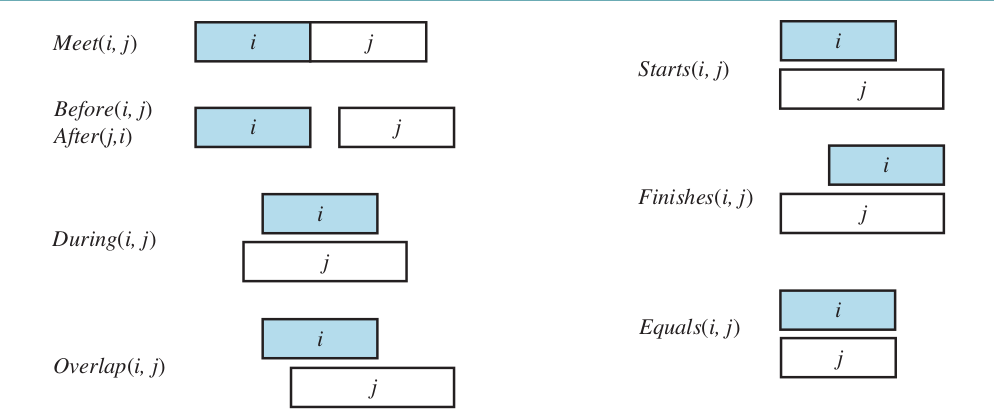
\includegraphics[width=0.95\textwidth]{images/allen-13-interval-logic.png}
	\end{center}
	\caption{}
	\label{fig: allen-13-interval-logic}
\end{figure} \footnote{
	These all have their intuitive meaning, with the exception of \textsc{Overlap}: we tend to think of
	overlap as symmetric (if $i$ overlaps $j$ then $j$ overlaps $i$), but in this definition, \textsc{Overlap}$(i, j)$
	only is true if $i$ begins before $j$ \cite{russell2016artificial}
}


% In this framework, time is modeled as \textit{linear} and \textit{infinite}, and the interval structure implies time is \textit{continuous}.

\begin{exmp} Allen's Interval Algebra

	\begin{enumerate}
		\item \textsc{During}($t_1$, $t_2$) time interval $t_1$ is fully contained within time interval $t_2$.

		\item \textsc{Starts}($t_1$, $t_2$) time interval $t_1$ shares a starting point with time interval $t_2$ but ends before $t_2$.

		\item \textsc{Finishes}($t_1$, $t_2$) time interval $t_1$ shares the same end as time interval $t_2$ but starts after $t_2$.

		\item \textsc{In}($t_1$, $t_2$) $\iff$ (\textsc{During}($t_1$, $t_2$) $\lor$ \textsc{Starts}($t_1$, $t_2$) $\lor$ \textsc{Finishes}($t_1$, $t_2$)).

		\item \textsc{Holds}(\(\phi\), \(t\)) is true iff \(\phi\) holds during \(t\).
	\end{enumerate}



	\begin{center}
		\textsc{Holds}(\(\phi\), \(T\)) \(\iff ( \forall t \) \textsc{In} $ (t,T) \implies $ \textsc{Holds}($\phi, t$)).
	\end{center}

	This definition states that \textsc{Holds}($\phi$, $T$) is true iff $\phi$ holds during every subinterval $t$ of $T$. In other words, $\phi$ holds throughout the entire interval $T$.
\end{exmp}

\begin{exmp} Complex logical expressions

	To allow properties to name complex logical expressions, there is a set of
	functions \textit{and}, \textit{or}, \textit{not}, \textit{all}, \textit{and} \textit{exists}, that correspond to the logical operators
	$\&, \lor, \sim, \forall$ and $\exists$ respectively.
	Conjunction moves through the HOLDS predicate freely:
	\begin{equation}
		\textsc{Holds}(\textsc{And}(p, q), t) \iff \textsc{Holds}(p, t) \  \& \  \textsc{Holds}(q, t)
	\end{equation}

	Negation is defined as follows:
	\begin{equation}
		\textsc{Holds}(\textsc{Not}(p), T) \iff (\forall t.\text{In}(t, T) \implies \sim \text{Holds}(p, t))
	\end{equation}
\end{exmp}




\subsection{Occurrences}
Allen uses three basic entities that are associated with time which are: \textit{properties}, \textit{events}, and \textit{processes}.
\begin{enumerate}
	\item \textbf{Events} describe an activity that involves an outcome. Examples of events such as ``John walked to the store''.

	\item \textbf{Processes} refer to some activity not associated with a result. Examples of processes include ``John was walking'' and ``John was running''.

	\item \textbf{Properties} are conditions that hold over a period of time. Examples of properties include ``John owns a cat''.
\end{enumerate}
One way to distinguish between \textit{events} and \textit{processes} is that one can count how many times an event occurs, but one cannot count
the number of times a process occurs.


The predicate \textsc{Occur} takes an event and a time interval and is true if the event happens over the time interval $t$ and there is no subinterval of $t$
over which the event occurs.

\begin{center}
	\textsc{Occur}($e$, $t$) $\land$ \textsc{In}($t^\prime$, $t$) $\implies$ \(\lnot\) \textsc{Occur}($e$, $t^\prime$).
\end{center}

Another way is to consider the characteristics of the set of temporal intervals that they hold or occur over.
Consider the \textit{process} ``I am walking'' over the Interval $I$. Unlike \textit{events}, this process might be occurring over subintervals of $I$ however a \textit{property} must be holding over every subinterval of $I$.


If a process $p$ took place over interval $t$ is denoted by the formula \textsc{Occurring}$(p,t)$.


As we illustrated, a process occurring over an interval $T$, must be occurring over at least one subinterval of $T$.\footnote{This process distinction is problematic, What does he mean by ``walking'' does not hold over all subintervals?
	\begin{itemize}
		\item
		      Does it mean that if we shoot a video of john walking, and watch the resulting walking picture one frame at a time, we would notice some frames we don't know he's ``walking'' or not?
		\item Or he mean while ``walking'' he might do something else?
	\end{itemize}
}

\section{Shoham Temporal Logic}

In his paper \cite{shoham1988temporal}.
Shoham shows how Allen' ontology has a problem defining the properties as they are not only not precise but they look like the \textit{First Order Predict Calculus}
($\mathcal{FOPC}$), so he missed the-off-shelf $\mathcal{FOPC}$.

Also, he shows that Allen's Ontology introduces unnecessary complexity just because Allen went for using intervals instead of time points.

Shoham states that the distinction between \textit{properties}, \textit{events}, and \textit{processes} is unnecessary and it's not very useful.
For example, much of Allen's discussion of event causation, \textsc{Ecause}, should apply to pairs of properties and mixed pairs of properties and events. Furthermore, this distinction is insufficient to express some other properties of propositions, such as that if a proposition holds over two overlapping intervals then it holds over
the union of the two intervals, though not necessarily vice versa (``I ran for more than two mile'').


\subsection{Shoham's Interval Logic}
Shoham has proposed using \textit{points} rather than \textit{intervals} as the basic temporal element and defines an interval as a pair of points.
\subsubsection{Syntax}
\begin{itemize}
	\item Given $TC$ a set of time points symbols,
	\item $C$ a set of constant symbols that's disjoint from $TC$;
	\item $TV$ a set of temporal variables,
	\item $V$ a set of variables that's disjoint from $TV$.
	\item $TF$ a set of temporal function symbols,
	\item $F$ a set of function symbols that's disjoint from $TF$.
	\item $R$ a set of relation symbols.
\end{itemize}

The set of temporal formulas is defined inductively as follows:
\begin{enumerate}
	\item All members of $TC$ are temporal terms.
	\item All members of $TV$ are temporal terms.
	\item if $trm_1, \dots, trm_n$ are temporal terms, and $f \in TF$ is an $n$-ary temporal function symbol, then $f(trm_1, \dots, trm_n)$ is a temporal term.
\end{enumerate}

The set of \textit{nontemporal formulas} is defined inductively in exactly the same way as the set of temporal formulas, with
$TC$ replace by $C$, $TV$ replaced by $V$, $TF$ replaced by $F$.

The set of well-formed formulas (wffs) is defined inductively as follows:
\begin{enumerate}
	\item if $trm_a$ and $trm_b$ are temporal terms, then $trm_a = trm_b$ and $trm_a \preceq trm_b$ are wffs.
	\item if $trm_a$ and $trm_b$ are temporal terms, $trm_1, \dots, trm_n$ are non-temporal terms, and $r \in R$ are n-ary relation symbol,
	      then
	      \[
		      \text{TRUE}(trm_a, trm_b, r(trm_1, \dots, trm_n))
	      \]
	      is a wff.
	\item if $\phi_1$ and $\phi_2$ are wffs, then $\phi_1 \land \phi_2$ and $\neg \phi_1$ are wffs.
	\item if $\phi$ is a wff and $z \in TV \cup V$ is a variable, then $\forall z \phi$ is a wff.
\end{enumerate}

Again, we assume the usual definition of $\lor, \exists, \equiv, \supset$, and so on.

\begin{exmp} Here's an example sentence.
	\begin{equation}
		\textsc{True}(t_1, t_2, \textsc{Color}(\textsc{House17}, \textsc{Red})))
	\end{equation}
	\begin{equation}
		\exists u \ \textsc{True}(t_3, t_4, \textsc{On}(u,B))
	\end{equation}
\end{exmp}

\subsubsection{Semantics}
An \textit{interpretation} is a tuple $\mathscr{S} = \langle  TW,\ \leqslant,\ W,\ TFN,\ FN,\ RL,\ M\rangle$ where $TW$
is a nonempty universe of time points, $\leqslant$ is a binary relation on $TW$, $W$ is a nonempty universe of individuals,
that is disjoint from $TW$, $TFN$ is a set of total functions $\bigcup_k (TW^k \rightarrow TW)$,
$FN$ is a set of total functions $ \bigcup_k (W^k \rightarrow W)$, $RL$ is a set of total relations over $W$, and
$M = \langle M1,\ M2,\ M3,\ M4,\ M5 \rangle$ is a meaning function as follows: $M_1 : T \rightarrow TW$,
$M_2: C \to W$, $M_3 : TF \to TFN$, $M_4 : TW \times TW \times F \to FN$, and $M_5: TW \times TW \times R \to RL$

A \textit{variable assignment} is a function $ VA = \langle VAT,\ VAV \rangle$, such that $VAT: VT \to TW$ and
$VAV: V \to W$. $M$ and $VA$ induce a time-dependent meaning $MVA$ on arbitrary terms in the following way.

We first define the meaning of arbitrary temporal terms. That meaning is the same regardless of when the terms are interpreted: the terms $1.1.2000$ and
$(12:00 + 12_{min})$ each denote a single, unambiguous absolute time. The precise
meaning of temporal terms is as follows. If $vt \in VT $, then $MVA (vt) = VAT (vt)$.
If $ct \in CT$, then $MVA (ct) = M_1(ct)$. If $f \in T F$ and $trm = f(trm_1, . . . , trm_n)$ Is a
the temporal term, then

\[
	MVA(trm) = M_3(f)(MVA(trm_1), \dots, MVA(trm_n))
\]

A more comprehensive ontology can be created by defining how the truth of a statement over a specific time interval is related to its truth over other related intervals.
The ontology includes several classes of temporal entities, such as \textit{Downward-hereditary} (which holds true overall subintervals), \textit{Upward-hereditary} (which holds true overall proper subintervals of some nonpoint interval, also holds over the nonpoint interval itself),
\textit{Liquid} (which is both upward- and downward-hereditary), \textit{Concatenable} (which holds true over the union of two consecutive intervals),
\textit{Gestalt} (which never holds true over two intervals, one of which contains the other), and \textit{Solid} (which never holds true over two overlapping intervals).

\begin{exmp} Examples
	\begin{enumerate}
		\item `The robot traveled less than two miles.'' is downward-hereditary.
		\item ``The robot traveled at a speed of two miles per hour'' is upward-hereditary.
		\item ``The robot started and ended at the same place'' and ``The robot traveled an even number of miles'' are concatenable.
		\item ``The robot executed the \textsc{Navigate} procedure (from start to finish)`` is solid.
	\end{enumerate}
\end{exmp}


\section{Galton Temporal Logic}
In his paper \cite{galton2004}, Galton has proposed a revision of Allen's temporal logic intended to represent continuous change.
His argument is that Allen's theory stands inadequate for representing continuous change because it requires the notion of \textit{instant} which is not captured by the notion of \textit{interval structure}.

\subsection{Properties and their negations}
In Allen's notation, the formula $\text{HOLDS}(p, T)$ says that the property $p$ holds over the interval $T$.
Allen introduces the axiom
\begin{equation}
	\textsc{Holds}(p, T) \leftrightarrow (\forall t) [\textsc{In}(t, T) \to \textsc{Holds}(p, t)].
\end{equation}
Allen follows this with a more complicated axiom:

\begin{equation}
	\textsc{Holds}(p, T) \leftrightarrow (\forall t) [\textsc{In}(t, T) \to (\exists s)[\textsc{In}(t, T) \land \textsc{Holds}(p, s)]].
	\label{eq:axiom1}
\end{equation}
And he defines the negation of a property as follows:
\begin{equation}
	\textsc{Holds}(\textsc{Not}(p), T) \leftrightarrow (\forall t) [\textsc{In}(t, T) \to \neg \textsc{Holds}(p, t)].
	\label{eq:axiom2}
\end{equation}
Allen notes that \textsc{Holds}(\textsc{Not}($p$, $T$)) implies $\neg$ \textsc{Holds}($p$, $T$), but not conversely, and that \textsc{Holds}(\textsc{Not}(\textsc{Not}($p$)), $T$) is equivalent to \textsc{Holds}($p$, $T$).

Galton shows that Allen's Axioms \ref{eq:axiom1} and \ref{eq:axiom2} lead to difficulties when dealing with continuous change.

\begin{exmp} \textit{property-negation} does not correctly capture what we understand by the negation of a property.

	Assume that \textit{property-negation} does exactly capture our intuitive understanding of the negation of a property. In that case, if we let $p$ stand for ``$X \  is \  at \ P$''
	then $not(p)$ must stand for ``$X \  is \  not \  at \ P$''.

	Now suppose that $X$ is in continuous motion throughout the interval $T$. This means that there is no subinterval of $T$ during which $X$ is at $P$;
	for if there were such a subinterval, then $X$ would be at rest throughout that subinterval, and hence not continuously moving throughout $T$.

	\begin{equation}
		\neg (\exists t)[\textsc{In}(t, T) \land \textsc{Holds}(p, t)]
	\end{equation}
	which is equivalent to
	\begin{equation}
		(\forall t)[\textsc{In}(t, T) \to \neg \textsc{Holds}(p, t)]
	\end{equation}
	and hence by (\ref{eq:axiom2}) is equivalent to
	\begin{equation}
		\textsc{Holds}(\textsc{Not}(p), T)
	\end{equation}
	By our assumption, this means that $X$ is not at $P$ throughout $T$. Since $P$ can be any point in space, this means that $X$ is never at any position at all at any time during $T$, which is absurd.

	The consequence is that in Allen's system, these properties are not really distinct; that is, Allen's system cannot distinguish between a body's being in a certain position and its being at rest there.
\end{exmp}

Galton gave more examples motivating his revision of Allen's temporal logic adding the notion of \textit{instant} to the theory to address the mentioned difficulties.

\subsection{Allen's interval logic needs instants}
Allen's argument for excluding \textit{instants} from his temporal ontology is, suppose we have two intervals $S$ and $T$ such that
\[
	\textsc{Meet}(S, T) \  \& \  \textsc{Holds}(p, S) \ \&  \ \textsc{Holds}(\textsc{not}(p), T)
\]
i.e $S$ and $T$ are contiguous intervals such that some proposition $p$ holds over $S$ and its negation holds over $T$. Then if we allow the existence of an instant $I$ at the point where $S$ and $T$ meet, one of the following cases must occur
\begin{enumerate}[label=(\arabic*)]
	\item  $I$ is part of both $S$ and $T$.\label{item:1}
	\item  $I$ is part of $S$ but not $T$.\label{item:2}
	\item  $I$ is part of $T$ but not $S$. \label{item:3}
	\item  $I$ is part of neither $S$ nor $T$. \label{item:4}
\end{enumerate}
In case \ref{item:1}, the proposition $p$ holds over $I$ and its negation holds over $I$, which is absurd;
in case \ref{item:2}, $p$ would be neither true nor false at $I$, which is absurd;
while as for the remaining two cases, since there's nothing to choose between them, any decision, either way, must be artificial. So, Allen concluded, we ought to banish instants altogether.

Galton states that the trouble is that Allen assumes that the only way we can embrace both instants and
intervals are by assuming that intervals are made up of instants, that instants are as it were the atoms out of which intervals are made.
Galton says the difficulty in the choice between \ref{item:1} to \ref{item:4} is because it has no relevance to real questions about time.

% Galton introduces  WITHIN$(I, T)$ that the instant $U$ falls within the interval $T$, and LIMITS$(I, t)$ to mean that $I$ limits $T$.
%
% He defines $ I = S*T$ as the instant $I$ is given as the meeting point of two contiguous intervals $S$ and $T$.
% He defines a proposition to hold over an instant $I$ as follows:
%
% $p$ holds at $I$ iff either neg($p$) holds throughout $S$ and throughout $T$ but not throughout JOIN$(S,T),$ where $I= S*T$ or $p$ holds throughout $T$ where $I$ falls within or limits $T$.
%
% Where 
% neg$(p)$ holds throughout $T$ iff it is not the case that $p$ holds throughout any subinterval of $T$.
%
% for on this definition, if $S$ meets $T$, it cannot happen that neg$(p)$ holds
% throughout $S$ and throughout $T$ but not throughout JOIN$(S, T)$. What we want,
% of course is a definition which, once "p holds at I" is defined, will yield the
% equivalence:
% neg $(p)$ holds at $I$ iff $p$ does not hold at $I$.

\subsection{States of position and states of motion}
Galton states that Allen's system can all be traced to the assumption, implicit throughout Allen's
work though never explicitly stated, that all properties should receive a
uniform treatment with respect to the logic of their temporal incidence. Our
starting point will therefore be to distinguish sharply between two kinds of
properties, having different temporal logics; I shall call these properties \textit{states
	of position} and \textit{states of motion}.

States of position can hold at isolated instants; and if a state of position
holds throughout an interval, then it must hold at the limits of that interval.
Examples: a body's being in a particular position, or moving at a particular
speed or in a particular direction. More generally, any state which consists of
some continuously variable quantity assuming a particular value is a state of
position.

States of motion cannot hold at isolated instants: if a state of motion holds
at an instant then it must hold throughout some interval within which that
instant falls. Examples: a body's being at rest or in motion, and more generally
any state of affairs which consists of some continuously variable quantity's
either remaining fixed or undergoing a change of value.

He then introduces
\begin{itemize}
	\item  \textsc{Holds-On}$(p, T)$ for a property $p$ to hold over an interval $T$.
	\item \textsc{Holds-In}$(p, T)$ for a property $p$ to during an interval $I$ (i.e. at some time during an interval not necessarily at the whole interval).
	\item \textsc{Holds-At}$(p, I)$ for a property $p$ to hold at an instant $I$.
\end{itemize}

For a property to hold during
an interval to be that there is at least one instant within the interval at which
the property holds,
\[
	\textsc{Holds-On}(p, T) \iff (\exists i)[\textsc{Within}(i, T) \  \& \ \textsc{Holds-At}(p, i)]
\]

and similarly, for a property to hold throughout an interval is for it to hold at
every instant within that interval:
\[
	\textsc{Holds-On}(p, T) \iff (\forall i)[\textsc{Within}(i, T) \  \to \textsc{Holds-At}(p, i)]
\]


\section{Versatile Event Logic (VEL)}
In \cite{bennett2001unifying}, they present formal semantics for a language representing temporal relationships and events, the language is called \textit{Versatile Event Logic }(VEL)

Unlike Allen, VEL uses both \textit{time points} and \textit{intervals variables} as well as \textit{tenses}.
Their formalism incorporates each of these:


\textbf{Events as transitions} A view of the event as a transition between states, this transition is handled by the modality
where a class of state transitions can be regarded as an accessibility relation.

\textbf{Events as occurrences over intervals}
Another approach to correlate events with the time intervals over which they occur.
This is done by means of a predicate \textsc{Occurs}$(e, \delta)$, which says that an event of type e occurs during
the interval $\delta$. Temporal relationships between events can then be described in terms of
relations between the intervals over which they occur, and in particular, by the 13 interval
relations of Allen \cite{allen1984towards}.

\textbf{Event radicals} representing events in terms of event radicals, syntactic
units which refer to \textit{event-types} and combine with temporal aspect operators to form
propositions. For example, if the event-type John-tie-his-shoelace were operated on by the
progressive aspect, we would obtain the proposition \textsc{Prog}(John-tie-his-shoelace), meaning
that an event of type ``John-tie-his-shoelace'' is in progress. We would read this as ``John is
tying his shoelace''.


\subsection{Temporal Ontology}
In VEL, In order to model all the possible states of the world which did not occur at any point in the actual
history of the world. They think of the set of all possible histories of the world as forming s branching tree structure.

\subsubsection{History structures}
To model the temporal order of states of an evolving universe and the relationship
between possible alternatives to the actual history of the world we employ a structure that
we call a \textit{History Structure}. This is a tuple $\mathcal{H} = \langle S, T, <, H \rangle$

\begin{itemize}
	\item $S$ is a set of world states.
	\item $T$ is a set of time points.
	\item $<$ is an irreflexive linear order on $T$.
	\item $H$ is a set of histories, each of which is a function from $T$ to $S$.
\end{itemize}

A pair $\langle \hbar_i, t_i \rangle$ (where $\hbar_i \in H$ and $t_i \in T$) is the \textit{index} of a possible world in the tree, and $h_i(t_i)$ denotes the world state that holds at that index.

An \textit{interval}$[t_1 \dots t_2]$ is the set $\{ t | t \in T \land t_1 \leq t \leq t_2\}$ of time points.


\subsubsection{States}
A world state $\hbar(t) \in S$ determines all properties of the world at time $t$ in history $\hbar$.

\subsubsection{Episodes}
In specifying the semantics for events, They referred to the interval in which an event occurs, also the history in which the event occurs.
Thus this lead to consider a pair $\langle \hbar, [t_1 \dots t_2] \rangle$
They define the \textit{episode} $[t_1 \dots t_2]_{\hbar}^{\approx}$ (where $t_1 \leq t_2$) by:
\[
	[t_1 \dots t_2]_{\hbar}^{\approx} = \{\langle \hbar^{\prime}, [t_1, \dots t_2] \ | \  \hbar^{\prime} \in H \land \hbar^{\prime} \approx^{t_2} \hbar \rangle\}.
\]

\subsubsection{Event-types}
An \textit{event-type} is a set of episodes. given the partial state $S^{\prime} \subseteq S$, the event-type
\[
	\{
	[t \dots t]_{\hbar}^{\approx} \ | \ (\exists t_1, t_2) [
			(t_1 < t < t_2) \land
			\]
			\[
			(\forall t^{\prime})[
					((t_1 < t^{\prime} < t) \to \hbar(t^{\prime}) \not\in S^{\prime}) \land
					((t \leq t^{\prime} \leq t_2) \to \hbar(t^{\prime}) \in S^{\prime})
				]
		]
	\}
\]

\subsubsection{Event-tokens}
\textit{Event-tokens} are occurrences of event-types.
an event-token as a pair $(\eta, e)$ where $\eta$ is a specific episode over which an event of type $e$ occurs, the proposed semantics provide a coherent framework that avoids the pitfalls of a naïve development of the idea that event-types can be regarded as predicates over a domain of event-tokens.

\subsubsection{Entities and individuals}
In a temporal language, \textit{individuals} must be able to persist through time even as their properties may change.
In the history tree model of time, an individual is realized in each world state by an \textit{entity}.
An individual is modeled by a function from states to entities, The time structure and the individuals that inhabit it are modeled by a VEL frame. This model does not impose any constraints on the set of entities or on the functions corresponding to individuals.
However, further constraints can be added to tie the theory to a particular model of reality.
Individuals are identified as functions from states to entities rather than using a more general model in which individuals are identified with functions from $H \times T$ to $S$. This identification seems to correspond to the way proper names are normally used.

\subsubsection{Verbs}
\textit{Verbs} are modeled as functions that take tuples of individuals as inputs and output event-types.
These verbs are treated as intensional, meaning their function also depends on the history and time at which they are evaluated.
\subsubsection{Propositions}
The VEL language's propositional expressions have a truth value that varies with history and time. To avoid pathological models, the truth value of a proposition cannot change infinitely often during a finite period. This is known as intermingling, and the prohibition of intermingling requires that a proposition's truth value is constant over open intervals of time.


\section{Conclusion}
We have seen different approaches to temporal representation and different reasoning,
Vendler has classified verbs based on their temporal behavior \textit{activities, accomplishments, achievements, states},
Allen has classified them into \textit{processes, events, and properties}.

We can see that Vendler's states are similar to Allen's properties, and Vendler's activities are similar to Allen's processes, and Vendler's accomplishments and achievements are similar to Allen's events.

\begin{table}[h]
	\centering
	\begin{tabular}{|c|c|}
		\hline
		\textbf{Vendler}                 & \textbf{Allen} \\
		\hline
		States                           & Properties     \\
		Activities                       & Processes      \\
		Accomplishments and Achievements & Events         \\
		\hline
	\end{tabular}
	\caption{Comparison of Vendler's and Allen's linguistic categories}
	\label{tab:comparison}
\end{table}

An important difference between Vendler's activities and Allen's processes is that Allen's process might be occurring over a subinterval of the interval,
Vendler defines this differently they describe processes as they consist of successive phases following one another in time.


Shoham propsed something different than Vendler and Allen, he proposed a temporal ontology, relying on the relation between the truth of the proposition
over one interval and its truth over others.

Galton divides Allen's states into two categories, \textit{states of postition} and \textit{states of mostion}.
